%% Versão final IEEE
%  \documentclass[journal]{IEEEtran}


% Versão edição no LATEX
\newcommand{\CLASSINPUTtoptextmargin}{2cm}
\newcommand{\CLASSINPUTbottomtextmargin}{2cm}
\documentclass[letter, onecolumn, 12pt]{IEEEtran} %journal


% Versão para impressão com margem maior para escrita
%  \documentclass[article,onecolumn, 11pt]{IEEEtran}
%  \usepackage[a4paper, marginparwidth=0.3in, 11pt]{geometry}


% \documentclass[journal,12pt,onecolumn]{IEEEtran}
% \usepackage[a4paper, marginparwidth=0.5in]{geometry}

% Versão Rascunho com uma coluna
%\documentclass[journal,12pt,onecolumn,draftclsnofoot,]{IEEEtran}
%\usepackage[a4paper, marginparwidth=1in]{geometry}

%



\usepackage[utf8]{inputenc}
% \usepackage{epstopdf}
%\usepackage[spanish]{babel}
\usepackage[cmex10]{amsmath,nccmath}
%\interdisplaylinepenalty=2500
\usepackage{amsfonts}
\usepackage{amssymb}
\usepackage{graphicx}
\usepackage{verbatim}
\usepackage{array}
%\usepackage{multirow}
\usepackage{subcaption}
\usepackage{dcolumn}
\usepackage{color}
\usepackage[noadjust]{cite}
\usepackage{url}
\usepackage{balance}
\usepackage[usenames,dvipsnames]{xcolor}
\usepackage{accents}
\usepackage{enumerate} % http://ctan.org/pkg/enumerate
\usepackage{blindtext}
%\usepackage{soul}
\usepackage[normalem]{ulem}
\usepackage{pgf,tikz}
% \usepackage{algpseudocode} 
% \usepackage{subfigure}
\usepackage{booktabs}
\usetikzlibrary{arrows}
%\DeclareGraphicsExtensions{.eps} % eu que comentei
%\AppendGraphicsExtensions{.pdf} % eu que comentei


% % % Adicionados por mim
%\usepackage[colorinlistoftodos]{todonotes}
\usepackage[colorinlistoftodos,prependcaption,textsize=small]{todonotes}
\usepackage{xargs} 

\newcommandx{\todoi}[2][1=]{\todo[linecolor=Plum,backgroundcolor=Plum!25,bordercolor=Plum,#1,inline]{#2}}
%\newcommand{\todop}[1]{\todo[textsize=tiny]{#1}}
%%%%



\DeclareMathOperator*{\Max}{max}
\DeclareMathOperator*{\Min}{min}
\DeclareMathOperator*{\argmin}{arg\,min}
\DeclareMathOperator*{\Maximize}{Maximize}

\begin{document}
\title{Wind Power Scenario Generation Using a High Dimensional Nonparametric Framework}

\author{Marcelo~Ruas~%,~\IEEEmembership{Student Member,~IEEE,}
	and Alexandre~Street%,~\IEEEmembership{Member,~IEEE}	
	
	
	%\thanks{This work was partially supported by UTE Parna\'iba Gera\c{c}\~ao de Energia S.A. through R\&D project ANEEL PD-7625-0001/2013.}
	%\thanks{Bruno Fanzeres, Arthur Brigatto and Alexandre Street are with the Electrical Engineering Department, Pontifical Catholic University of Rio de Janeiro (PUC-Rio), Rio de Janeiro, RJ, Brazil (e-mail: \mbox{bsantos@ele.puc-rio.br}; \mbox{street@ele.puc-rio.br}).}
	%\thanks{L. A. Barroso are with PSR Consulting, Rio de Janeiro, RJ, Brazil (e-mail: \mbox{luiz@psr-inc.com}).}
}

\maketitle


\begin{abstract}
	Producing probabilistic forecasts of Renewable Generation is a topic of interest in power system applications. In this work, we focus on generating future scenarios of wind power generation.  Most time series methods used to produce such forecasts rely on the assumption of Gaussian errors or Gaussian distribution, however applications on power systems deals with nongaussian time series.  
	We develop, in this work, a nonparametric methodology based on Quantile Regression to estimate the conditional distribution function for monthly wind time series.  
	The conditional distribution is formed by connecting an array of quantiles jointly estimated. 
	Two different models are used to estimate the quantiles: (i) the model Quantile Regularized Adaptive LASSO (QRAL) and (ii) the Nonparametric Quantile Regression (NQR) model.
	The QRAL implements two types of regularization. One is based on the Adaptive LASSO for selecting covariates within each Quantile Regression. The other emphasizes the connection across different quantiles, reflecting the fact that the quantile function should have smooth variation. Quantile function has to variate smoothly across quantiles and it is implemented by the addition of a second derivative filter, 
exploring the similarity of neighbor quantiles. The NQR model allows nonlinear functions of its covariates. Each nonlinear function is a continuous function penalized by its second derivative.
	A case study with realistic Wind Power data from the Brazilian Northeast compares the  with different benchmarks in the literature. The QRAL was able to outperform them in terms of minimizing the Mean Absolute Percentile Error of future scenarios in recovering the historic monthly quantiles. The NQR method is under development.
\end{abstract}

\begin{IEEEkeywords}
	Quantile Regression, Model Identification, Non-gaussian time series model
\end{IEEEkeywords}


%\listoftodos


% ===== Sec. I - Introduction ===== %

\section{Introduction}

%%%%%%% 1. Talk about renewable energy and its variability - motivacao da importancia do estudo da probability forecasting OK

Renewable energy power is an emergent topic which is demanding attention from the academic community. %It is a much cleaner way of producing energy than by using other sources such as coal and gas, and with less hazard potential than nuclear power plants. 
The installed capacity of renewable energy plants has been increasing in a fast pace and projections point out that wind power alone will account to 18\% of global power by 2050  \cite{IntEnerAgency}.
In spite of its virtues, several new challenges are inherent when dealing with such power source, due to its unpredictability. To overcome this lack of certainty, one has to work with many different possibilities of outcome.

%Many applications in Power Systems use renewable scenarios as input.
%For all the aforementioned applications, the knowledge of the time series conditional distribution can provide all that needed information.
New statistical models capable of handling such difficulties are an emerging field in power systems literature \cite{zhang_review_2014 , bessa2012time, gallego2016line,moller_time-adaptive_2008,nielsen2006,bremnes_probabilistic_2004,wan_direct_2017} 
The main objective in such literature is to propose new models capable of generating scenarios of renewable generation (RG) which are demanded in (i) energy trading, (ii) unit commitment, (iii) grid expansion planning, and (iv) investment decisions (see (\cite{moreiraStreet,jabr2013robust,zhaoguan,Aderson2017}) and references therein). 
In stochastic optimization, problems such as Unit Commitment, Economic Dispatch, Transmission Expansion Planning all use scenarios as input. 
Such scenarios are used to characterize the probability distribution within the optimization under uncertainty framework.
When working with robust optimization, bounds for probable ranges of coefficients are needed.

%%%%%% 1.b. Continuar 
%It is important to have good forecasts of either high and low quantiles to to measure the probability of extreme scenarios. 
%the complex behavior of wind is very difficult to model and predict.  \todo{Melhorar esta parte? "é importante prever bem quantis altos e baixos p analise de risco - fica prejudicada pela dificuldade de previsao destes quantis"}
%Having better prediction models can help the planner to make better and less risky decisions, increasing the attractiveness of renewable energy to the energy system. 
%In this work we will investigate how to model dynamics of renewable energy time series in both short and long terms.
 
%%%%%%%% 2. Falar de Wind Power nos primordios. ARIMA e essas coisas
% Henrique faz Critics about point forecasts and gaussian models (ARIMA-GARCH). Compare GAS and nonparametric models.

%% Eu faço a introdução ao probabilistic forecasting
Conventional statistical models are often focused on estimating the conditional mean of a given random variable. % This is not very useful when dealing with renewable energy, as the variability and the notion of risk is extremely important for planning. - ver a distribuicao como um todo - reescrever
%One of the first works in wind power prediction, \cite{brown_time_1984} treated the nonlinearity of wind power by applying a transformation on the prediction of wind speed, which is modeled by an autoregressive process. The data is standardized to account for the normal variation during the day.
%\cite{moeanaddin_numerical_1990} estimated the $k$-step-ahead conditional density function using the Chapman-Kolmorov relation. The method is applied on a non-linear autoregressive time series.
By reducing the outcome to a single statistic, we loose important informations about the time series random behavior. In order to account for the process inherent variability it is important to consider probability forecasting.
In \cite{zhang_review_2014}, reviews the commonly used methodologies regarding probabilistic forecasting models, splitting them in parametric and nonparametric classes. Main characteristics of \textbf{parametric models} are (i) assuming a distribution shape and (ii) low computational costs. ARIMA-GARCH, for example, model the RG series by assuming the distribution \textit{a priori}. On the other hand, \textbf{nonparametric models} (i) don't require a distribution to be specified, (ii) needs more data to produce a good approximation and (iii) have a higher computational cost. Popular methods are Quantile Regression (QR), Kernel Density Estimation,  Artificial Intelligence or a mix of them.


%%%%%% 3. Falar da não-gaussianidade do WP e apresentar novas referências
% Unir com parágrafo anterior??
% Não gaussianidade dos dados de Fator de capacidade eólico 3 paragrafo HHH
Most time series methods rely on the assumption of Gaussian errors. However, RG time series such as wind and solar are reported as non-Gaussian \cite{bessa2012time,jeon2012using,taylor2015forecasting,Wan2017}. To circumvent this problem, the usage of nonparametric methods - which does not rely on assuming any previously assumed distribution - is adequate. 
Quantile Regression (QR) is a tool for constructing a methodology for non-gaussian time series, because of its facility to implement on commercial solvers and to extend the original model.
However, when estimating a distribution function, as each quantile is estimated independently, the monotonicity of the distribution function may be violated.
This issue - also known as crossing quantiles - can be adressed by constraining the sequence of quantiles to be in an increasing order. Other possibility is making a transformation afterwards, as shown in \cite{chernozhukov_quantile_2010}.

%
%, as defined in \cite{koenker_quantile_2006}.

%%%%% 4. Falar de regressao quantilica em geral. Onde é utilizada e etc.


The seminal work \cite{koenker1978regression} defines QR as we use today. By this formulation, the conditional quantile is the solution of an optimization problem where we minimize the sum of the check function (defined formally in the next session). Instead of using the classical regression to estimate the conditional mean, the QR determines any quantile from the conditional distribution. Applications are enormous, ranging from risk measuring at financial funds (the Value-at-Risk) to a central measure robust to outliers.
By estimating many quantiles on a thin grid of probabilities, one can have as many points as desired from the estimated conditional distribution function. 
In \cite{koenker_quantile_2006}, the application of QR is extended to time series, when the covariates are lagged values of $y_t$.  
In our work, beyond autoregressive terms, it is also considered other exogenous variables as covariates. 



%%%%% 5. aplicações de QR em wind power, colocando os papers mais proximos.
% colocar tb regressao quantilica com regularizacao
In \cite{gallego2016line,moller_time-adaptive_2008,nielsen2006,bremnes_probabilistic_2004,wan_direct_2017}, QR is employed to model the conditional distribution of Wind Power Time Series.
An updating quantile regression model is presented by \cite{moller_time-adaptive_2008}. The authors present a modified version of the simplex algorithm to incorporate new observations without restarting the optimization procedure.
%Using existing wind power forecasting to extend these forecasting to build a model of quantiles is the strategy adopted by \cite{nielsen2006}.
In \cite{nielsen2006}, the authors build a quantile model from already existent independent Wind Power forecasts.
The approach by \cite{gallego2016line} is to use QR with a nonparametric methodology. The authors add a penalty term based on the Reproducing Kernel Hilbert Space, which allows a nonlinear relationship between the explanatory variables and the output. This paper also develops an on-line learning technique, where the model is easily updated after each new observation.
In \cite{wan_direct_2017}, wind power probabilistic forecasts are made by using QR with a special type of Neural Network (NN) with one hidden layer, called extreme learning machine. In this setup, each quantile is a different linear combination of the features of the hidden layer.
The authors of \cite{cai_regression_2002} use the weighted Nadaraya-Watson to estimate the conditional function in the time series.

Regularization is a topic already explored in previous QR papers.
The work by \cite{belloni_l1-penalized_2009} defines the properties and convergence rates for QR when adding a penalty proportional to the $\ell_1$-norm to perform variable selection, using the same idea as the LASSO \cite{tibshirani1996regression}. The ADALASSO equivalent to QR has its properties investigated by \cite{ciuperca_adaptive_2016}. In this variant, the penalty for each variable has a different weight, and this modification ensures that the oracle property is being respected. 
In \cite{zou_regularized_2008,jiang_interquantile_2014}, the AdaLASSO is employed to QR with multiple quantile regressions at the same time, relating the estimated coefficients of different quantiles.

In this work we propose the use of a non parametric technique, which as already mentioned is free from user distribuitional specification, to simulate future scenarios of wind power generation. Such technique relies on a quantile autoregressive (QAR) framework in the same spirit as \cite{koenker1978regression,koenker_quantile_2006,koenker2005quantile}. Notwithstanding, as an innovation from the referenced works, in order to capture which variables would improve model fit, from a set of relevant ones, we propose the use of a LASSO cost function plus an interquantile term. Such term acts as a filter to impose coefficient stability for a given covariate across the set of quantiles. In addition, interquantile dependency is explored as in \cite{zou_regularized_2008,jiang_interquantile_2014}. As a second innovative feature of this work, we propose the inclusion of a penalization parameter in the second difference. We argue that such strategy avoids extreme quantiles to be shrinked to zero as fast as the central ones. For the best of the authors knowledge, no other work has developed a methodology where regularization and estimation of the conditional distribution using QR is carried on at the same time with the objective of generating future scenarios for WPG time series.

%The crossing quantile issue is solved by introducing a constraint on the optimization problems that forces the quantile function monotonicity. Furthermore, in the quantile regression literature for wind forecasting, a sequence of quantiles is provided as output. In our work, we propose to estimate the conditional distribution as a whole.


 
%%%%%% 7. Objetivos do paper e contribuição
The objective of this paper is, then, to propose a new methodology to address nonparametric time-series model focused on RG. This may be seen as a multiple quantile regression problem that specifies a time series model based on the empirical conditional distribution. The main contributions are:
\begin{itemize}
	\item A nonparametric methodology to model the conditional distribution of RG time series to produce scenarios.
	
	\item The proposition of a methodology that selects the global optimal solution with parsimony both on the selection of covariates as on the quantiles. This methodology is based on the Adaptive LASSO for QR (Linear Programming).
	
	\item Regularization techniques applied to an ensemble of quantile functions to estimate the conditional distribution, solving the issue of non-crossing quantiles. On regularizing quantiles, we propose a smoothness on the coefficient value across the sequence of quantiles.	
	%\item A nonlinear QR
	
\end{itemize}

%We propose a new combination of methods to predict the $k$-step ahead conditional distribution. By using MILP, we achieve a solution which is optimal for the given objective. In order to improve the quality of predictions and interpretability, we incorporate a joint regularization by specifying the existence of groups among the probabilities $\alpha$. We could not find any other work in the literature that interpreted different quantiles as models depending on one another. 
%The objective of this paper is to propose and test different techniques of predicting the conditional distribution based on QR. 


% OBJETIVOS:
%Um modelo para séries tmeporais autoregressivo e nao parametrico e baseado na função quantilica. No caso autoregressivo, uma metodologia de estimação com seleção parcimoniosa otima global é proposta e possibilita o controle dos números de grupos de regressores diferentes dentro do modelo para diferentes quantis. Para o modelo não paramétrico
%Modelo data driven, empirico


%%%%%% 8. Organização dos próximos capítulos OK
The remaining of the paper is organized as follows. In section II, we present the quantile regression framework in which we build the model as well as introduce the Quantile Regression Adaptive LASSO. In section III, we discuss the estimation procedures for them. The regularization strategies are also presented on this section. Finally, in section IV, we present a few controlled studies with simulated data and a final case study using real data from wind power is presented in order to test our methodology. Section V will conclude this article.


% ===== Sec. II - Quantile Regression ===== %
%
\section{Quantile Regression based time series model} \label{sec:qr1}

Let the $\alpha$-conditional quantile function of $Y$ for a given value $x$ of the $d$-dimensional random variable $X$, i.e., $Q_{Y|X}:[0,1] \times \mathbb{R}^d \rightarrow \mathbb{R}$, can be defined as %(in short, from now on, $Q_{Y|X}(\cdot, \cdot)$)
	\begin{equation}
	Q_{Y|X}(\alpha,x) = F_{Y|X=x}^{-1}(\alpha) = \inf\{y: F_{Y|X=x}(y) \geq \alpha\}.
	\label{eq:quantile-function}
	\end{equation}
The Conditional Quantile Function $Q$ is the inverse of the Distribution Function $F$, and represents the smallest value $y$ for which the distribution function is greater than a given probability $\alpha$.

Let $\rho$ be the check function 
	\begin{equation}\label{eq:check-function}
	\rho_{\alpha}(x)=\begin{cases}
	\alpha x & \text{if }x\geq0\\
	(1-\alpha)x & \text{if }x<0
	\end{cases}.
	\end{equation}
The quantile function for a given finite sample $\{y_t,x_t \}_{t \in T}$, where $T$  is the set of time indexes, and a given probability $\alpha$ is the solution of minimizing the loss function $L_\alpha(\cdot)$:
	\begin{IEEEeqnarray}{C}
	\hat{Q}_{Y|X}(\alpha,\cdot)\quad\in\quad  \underset{q\in\mathcal{Q}}{\text{arg min}}\, L_\alpha(q) = \sum_{t\in T}\rho_{\alpha}(y_{t}-q(x_t)).\label{eq:optim-lqr1} 
	\end{IEEEeqnarray}
For Inference on Quantile Regression and finite sample properties, see the Chapter 3 on \cite{koenker2005quantile}.
The $\alpha$-quantile function $q(\cdot)$ belongs to a function space $\mathcal{Q}$. We might have different assumptions for space $\mathcal{Q}$, depending on the type of function we want to find 
for $q$. A few properties, however, must be achieved by our choice of space, such as being continuous and having limited first derivative. In this work, we consider the following two cases: 
\begin{enumerate}
	\item $\mathcal{Q}$ is a linear function space such that
		$q_\alpha(x_t) = \beta_0 + \beta^T x_t;$ 
	\item $\mathcal{Q}$ is a space of continuous functions with limited first and second derivatives.
\end{enumerate}

% Let the finite discretization of the interval $[0,1]$ be composed of a sequence of probabilities $0 < \alpha_1 < \alpha_2 < \dots < \alpha_{|J|} < 1$ and denote as $A$ the set $A = \{ \alpha_j \mid j \in J \}$, where $J$ is an index set for the probabilities $\alpha$.
% In the next subsections\todo{se fala assim?}, we present in more details how to use the two aforementioned hypothesis for $\mathcal{Q}$ and estimate a sequence of quantiles $\{ q_{\alpha_j} \}_{j\in J}$. 


\subsection{Linear Model}

The linear model presumes that the $\alpha$-quantile function is a linear function of its regressors:
$$q_{\alpha}(x_t) = \beta_{0} + \beta^T x_t.$$   
When dealing with many candidates of covariates, one has to deal with the problem of selecting the relevant ones out of a set of candidates which improve model fit. In practice, it means that some coefficients from the vector $\beta = [ \beta_{1 } \cdots \beta_{p} ]$ might assume zero value.
There are many ways of selecting a subset of variables among the available options.
A classical approach for this problem is the Stepwise algorithm \cite{efroymson1960multiple}, \cite{hocking_selection_1967}, \cite{tibshirani1996regression}, which includes variables in sequence. 

A popular way of variable selection which fits on a linear programming context are the LASSO/AdaLASSO techniques, which consists in penalizing the $\ell_1$-norm. Besides shrinking coefficients towards to zero, it has also the capability of effectively pushing coefficients to zero (an effect that ridge regression cannot achieve \cite{tibshirani1996regression}). The usage of LASSO and AdaLASSO in QR context is the topic of study in \cite{li_l1-norm_2008,ciuperca_adaptive_2016,belloni_l1-penalized_2009,zou_regularized_2008,jiang_interquantile_2014}.
We refer to the reader the work from \cite{belloni_l1-penalized_2009}, where it is possible to find specific properties and convergence rates when using the LASSO to perform model selection in a quantile regression framework. 

Regarding the penalization parameter $\lambda$, which dictates the shrinkage magnitude of the linear coefficients, the level of parsimony of the model can be defined by the user through such quantity. This is due to the fact that higher values of $\lambda$ means less variables selected to be non-zero. 

The single $\alpha$-quantile AdaLASSO is estimated by the following optimization problem:
\begin{IEEEeqnarray}{c}
\underset{\beta_{0},\beta}{\text{min}} \sum_{t \in T} \rho_\alpha(y_t - (\beta_0 + \sum_{p \in P} \beta_p x_{tp})) +\lambda \sum_{p \in P} w_p | \beta_p |.\label{eq:l1-qar-optim} 
\end{IEEEeqnarray}
What differs the AdaLASSO from the LASSO is the inclusion of the term $w_p$. Suppose the model (\ref{eq:l1-qar-optim}) is estimated with all $w_{p}=1$, the output of the optimization problem are coefficients of LASSO  $\beta^{L}_{p}$. The AdaLASSO coefficients $\beta^{AL}_{p}$ are obtained when solving the same optimization problem while letting $w_{p}=1/|\beta^{L}_{p}|$. 
% What differs the AdaLASSO from the LASSO is the inclusion of the term $w_p$. Suppose the model (\ref{eq:l1-qar-optim}) is estimated with all $w_{pj}=1$, the output of the optimization problem are coefficients of LASSO  $\beta^{L}_{pj}$. The AdaLASSO coefficients $\beta^{AL}_{pj}$ are obtained when solving the same optimization problem while letting $w_{pj}=1/|\beta^{L}_{pj}|$. % para voltar o 'j'






\subsection{Nonparametric Quantile Regression}
\label{sec:npqar}

Fitting a linear estimator for the QR is less attractive when nonlinearity is present in the quantile functions. In Figure \ref{fig:nonlinear}, a nonlinear relationship between variables $x$ and $y$ is presented, where $y = x^2 + error$. When using a linear estimator for this type of relation, this estimator underestimates the quantile for a chunk of data while overestimating for the other chunk. In cases such as this, a nonlinear estimator for the quantiles produces better results.
\begin{figure}[t]
	\begin{center}
	  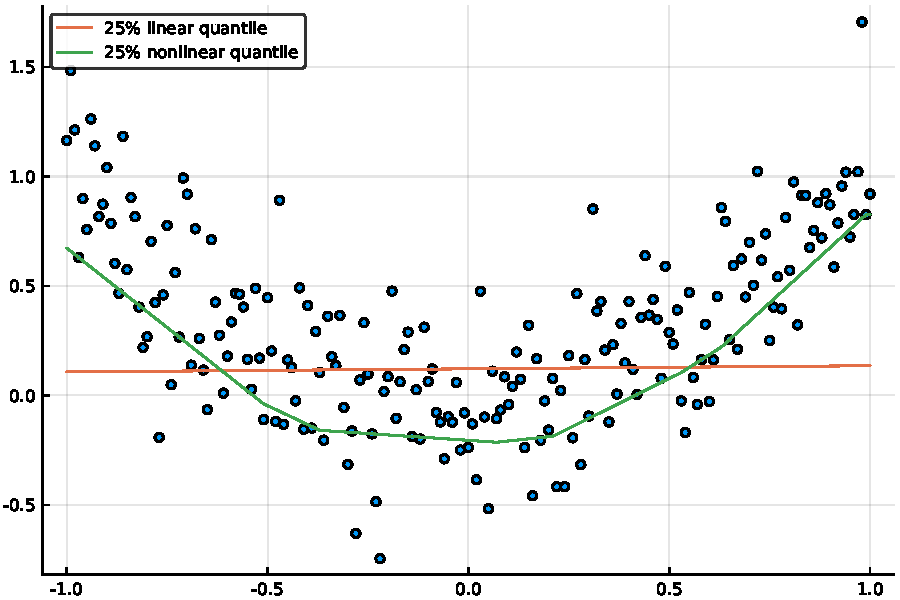
\includegraphics[width=0.7\textwidth]{Images/nonlinear}
	\end{center}
	\caption{Calculating the 25\% quantile with both methodologies when there is a nonlinear relationship between $x$ and $y$. While the linear estimator fails to estimate the conditional quantile, the nonlinear estimator is able to capture the quadratic dependency.}
	\label{fig:nonlinear}
\end{figure}
Comparing both quantile estimator, it is clear that the nonparametric is capable of capturing the nonlinearity on the relationship, while the linear model can only capture linear relationships.

A nonlinear estimator is built by allowing the quantile function $q(\cdot)$ to freely adjust to the data. The only required aspects for $q$ are being continuous and having limited first and second derivatives.
In order to acomplish this, we introduce a Nonparametric Quantile Autoregressive model with a $\ell_{1}$-penalty term on both the first and second derivatives, represented by their discrete aproximation $D^1 q_t$ and $D^2 q_t$ on equations (\ref{eq:d1qt}) and (\ref{eq:d2qt}), respectively, presented below:
\begin{equation}
  D^{1}_{tj}=\frac{q_{t+1}-q_{tj}}{x_{t+1}-x_{t}},\label{eq:d1qt}
\end{equation}
\begin{equation}
D_{x_{t}}^{2}q_{t}=\frac{\left(\frac{q_{t+1}-q_{t}}{x_{t+1}-x_{t}}\right)-\left(\frac{q_{t}-q_{t-1}}{x_{t}-x_{t-1}}\right)}{x_{t+1}- x_{t-1}}.\label{eq:d2qt}
\end{equation}


% To prevent overfitting and smoothen our predictor, we include a penalty on its roughness by including the $\ell_1$ norm of its second derivative. For more information on the $\ell_1$ norm acting as a filter, one can refer to \cite{kim2009ell_1}.

% This time, as opposed to when employing linear models, we don't suppose any functional form for $q_\alpha(x_t)$. This forces us to build each $q_\alpha$ differently: instead of finding a set of parameters that fully defines the function, we find a value for $q_\alpha(x_t)$ at each instant $t$. On the optimization problem, we will find optimal values for a variable $q_{tj} \in \mathbb{R}$, each consisting of a single point. The sequence  $\{ q^*_{\alpha t} \}_{\alpha \in A} $ will provide a discretization for the quantile function $\hat{q}_\alpha(x_t)$, which can be found by interpolating these points.

% notação estatística de ordem. com x^(0)


Let $\{\tilde{y}_t \}_{t=1}^n$ be the sequence of observations in time $t$ and let $\tilde{x}_t$ be the $p-$lagged time series of $\tilde{y}_t$, such that $\tilde{x}_t = L^p(\tilde{y}_t)$, where $L$ is the lag operator. Matching each observation $\tilde{y}_t$ with its $p-$lagged correspondent $\tilde{x}_t$ produces $n-p$ pairs $\{(\tilde{y}_t,\tilde{x}_t)\}_{t=p+1}^n$ (note that the first $p$ observations of $y_t$ must be discarded). When the sequence of observations of $x$ are reorder in such a way that they are in growing order
$$\tilde{x}^{(p+1)} \leq \tilde{x}^{(p+2)} \leq \dots \leq \tilde{x}^{(n)},$$ 
the new sequences can be defined $\{x_i\}_{i=1}^{n-p} = \{\tilde{x}^{(t)} \}_{t=p+1}^{n}$ and $\{y_i\}_{i=1}^{n-p} = \{\tilde{y}^{(t)} \}_{t=p+1}^{n}$, where $T' = \{2,\dots, n-p-1\}$. 
% The optimization model to estimate the nonparametric quantile is as follows:
% \begin{equation}
% \begin{split}
% \hat{q}_{\alpha_j}(x_t) =\underset{q_{tj}}{\arg\min}\sum_{t\in T'} \rho_{\alpha_j} \left( y - q_{tj} \right) \\ +\lambda_1  \sum_{t\in T'}|D_{x_t}^{1}q_{tj}| +\lambda_2  \sum_{t\in T'}|D_{x_t}^{2}q_{tj}|,
% \end{split}
% \end{equation}
% where $D^1 q_t$ and $D^2 q_t$ are the first and second derivatives of the $q_\alpha(x_t)$ function, calculated as follows:
% \begin{equation*}
% D_{x_{t}}^{2}q_{tj}=\frac{\left(\frac{q_{\alpha t+1}-q_{tj}}{x_{t+1}-x_{t}}\right)-\left(\frac{q_{tj}-q_{\alpha t-1}}{x_{t}-x_{t-1}}\right)}{x_{t+1}- x_{t-1}},
% \end{equation*}
The optimization model to estimate the $\alpha$-quantile nonparametrically is as follows:
\begin{equation}
\begin{split}
\hat{q}_{\alpha}(x_t) =\underset{q_{t}}{\arg\min}\sum_{t\in T'} \rho_{\alpha} \left( y - q_{t} \right) \\ +\lambda_1  \sum_{t\in T'}|D_{x_t}^{1}q_{t}| +\lambda_2  \sum_{t\in T'}|D_{x_t}^{2}q_{t}|.
\end{split}
\end{equation}
The purpose of the filters, then, is to control the amount of variation for the estimator $q_\alpha(x_t)$. When no penalty is employed, the estimated quantile always match the observations $q_{tj} = y_t$, for any given $\alpha$. On the other hand, when $\lambda_2 \rightarrow \infty$, the estimator approaches the linear quantile regression. 

%The first part on the objective function is the usual Loss function for $\{q_{t\alpha}\}_{\alpha \in A}$. The second part are the $\ell_1$-filters. The purpose of the filters is to control the amount of variation for the estimator $q_\alpha(x_t)$. When no penalty is employed we would always get $q_{tj} = y_t$, for any given $\alpha$. On the other hand, when $\lambda_2 \rightarrow \infty$, our estimator approaches the linear quantile regression. 








\section{conditional distribution based on Quantile Regression for Time Series}

In the previous section, we presented two methods for estimating a single $\alpha$-quantile by using QR. However, to build a CDF from an array of quantile, we propose to jointly estimate them, in order to explore the connection across different quantiles. 

Let the finite discretization of the interval $[0,1]$ be composed of a sequence of probabilities $0 < \alpha_1 < \alpha_2 < \dots < \alpha_{|J|} < 1$ and denote as $A$ the set $A = \{ \alpha_j \mid j \in J \}$, where $J$ is an index set for the probabilities $\alpha$. 
The $\alpha$-quantiles are, from this point forward, indexed by $j$, to account for the different models that are simultaneously estimated. A property that must be respected is the monotonicity of the Quantile function $Q$, such that $q_{\alpha_1} \leq q_{\alpha_2} \dots \leq q_{\alpha_{|J|}}$.
The sequence of quantiles define a continuous quantile function after interpolation, and finally a CDF after inverting the estimated quantile function.

The following subsections present how to jointly estimate quantiles through QR for each one of the two methods.
% To estimate the conditional distribution, $\hat{Q}_{Y_{t+h}|X_{t+h},Y_t, Y_{t-1}, \dots} (\alpha,\cdot)$, of time series $\{y_t\}_{t \in T}$ $h$-steps ahead, where $X_{t+h}$ makes reference to a vector of exogenous variables. Once the conditional distribution is estimated, future scenarios can be obtained by simulation. %In this paper, we focus on the 1-step ahead forecasting ($h=1$) and the model don't include any covariates but its own autoregressive terms. 



\subsection{Linear Model}

As we are interested on the conditional distribution as a whole, we estimate multiple quantiles at once. In order to produce a coherent distribution function, the output of the problem must respect certain properties, such as being monotone increasing. 
Besides that, one can expect that the value of similar quantiles be produced by similar models. If the coefficient of a given $p$ covariate changes too abruptly with respect to a change on the probability $\alpha$, there is a high probability that the estimation did not produce good results rather than this noise belonging to the true model.  In order to correct this much common behavior in QR estimation, we introduce a second derivative filter,given by the discrete approximation shown below:
\begin{equation}
D_{pj}^{2}:=\frac{\left(\frac{\beta_{p,j+1}-\beta_{pj}}{\alpha_{j+1}-\alpha_{j}}\right)-\left(\frac{\beta_{p,j}-\beta_{p,j-1}}{\alpha_{j}-\alpha_{j-1}}\right)}{\alpha_{j+1}-\alpha_{j-1}}.
\end{equation}
With this approach, one can keep track on the crossing quantiles issue as well as using a interquartile structure as a strategy to reduce noise on estimation %! explicar melhor o porquê
The works by \cite{zou_regularized_2008, jiang_interquantile_2014} also use multiple quantile regressions at once and make use of interquantile similarities to produce regularization on the quantiles. In \cite{zou_regularized_2008}, the author uses the norm $\| \beta \|_{1\infty}=\sum_{p=1}^{|P|} \max\{ |\beta_j^{(k)} |\}$ as penalization. Such penalization is imposed on the maximum value among all quantiles for a given covariate. This idea is extended by \cite{jiang_interquantile_2014}, that uses a fused AdaLASSO mixing the LASSO penalization with the absolute interquantile difference.

The statistical model \textbf{Quantile Regularized Adaptive LASSO (QRAL)} is defined by the vector of coefficients $\beta_{0}$ and the matrix of size $|P| \times |J|$ of regressor coefficients $\beta_{pj}$. These coefficients are the solution from the minimization problem given below:
% \begin{IEEEeqnarray}{lr}  % para duas colunas
% 	\underset{\beta_{0j},\beta_j}{\text{min}} \sum_{j \in J} \left( \sum_{t\in T}\rho_{\alpha_j}(y_{t}-(\beta_{0j} + \beta_j^T x_t)) \right.  \span \nonumber \\
% 	\span \left. + \lambda\  \sum_{p \in P} w_{pj}^\delta \mid  \beta_{pj} \mid \right) + \gamma \sum_{p \in P} \sum_{j \in J'} |D^2_{pj}|,\label{eq:adalasso_model}
% \end{IEEEeqnarray}
\begin{IEEEeqnarray}{lr} % para uma coluna
	\underset{\beta_{0j},\beta_j}{\text{min}} \sum_{j \in J} \left( \sum_{t\in T}\rho_{\alpha_j}(y_{t}-(\beta_{0j} + \beta_j^T x_t)) \right.   \left. + \lambda\  \sum_{p \in P} w_{pj}^\delta \mid  \beta_{pj} \mid \right) + \gamma \sum_{p \in P} \sum_{j \in J'} |D^2_{pj}|, \span \label{eq:adalasso_model_mat1}\\
	\text{subject to} \span \nonumber \\
	\beta_{0j} + \beta_{j}^T x_{t} \leq \beta_{0,j+1} + \beta_{j+1}^T x_{t},& \forall t \in T, \forall j \in J_{(-1)},\label{eq:adalasso_model_mat2} 
\end{IEEEeqnarray}
where the weights $w_{pj} = 1/\tilde{\beta}_{pj}$ and $\tilde \beta_{pj}$ are the coefficients from the first-step LASSO estimation. The parameter $\delta$ is an exponential parameter usually set to 1.
The sum of absolute values that compose the second derivative filter $\sum_{j \in J'}\sum_{p \in P}|D_{pj}^{2}|$ is added on the objective function multiplied by a tuning parameter $\gamma$, where the set $J'=\{2,\dots,|J|-1 \}$.

\subsection{Nonparametric Quantile Regression}

%The quantile estimation is done for different values of $\lambda_2$. By using different levels of penalization on the second difference, the estimation can be more or less adaptive to the fluctuation. It is important to notice that the usage of the $\ell_1$-norm as penalty leads to a piecewise linear solution $q_{t \alpha}$. % Referenciar?

To jointly estimate multiple quantiles, the optimization problem that defines NQR is changed to the following:
\begin{IEEEeqnarray}{lr}
\underset{q_{tj}}{\min} \sum_{j \in J} \left( \sum_{t\in T'} \rho_{\alpha_j} \left( y - q_{tj} \right)  +\lambda_1  \sum_{t\in T'}|D_{x_t}^{1}q_{tj}| +\lambda_2  \sum_{t\in T'}|D_{x_t}^{2}q_{tj}| \right), \span \label{eq:nqr-mat1} \\
\text{subject to} \span \nonumber \\
q_{t j} \leq q_{t j+1}, &  \forall t \in T, \forall j \in J_{(-1)},\label{eq:nqr-mat2}
\end{IEEEeqnarray}
where equation (\ref{eq:nqr-mat2}) is a noncrossing constraint.

Figure \ref{fig:npqar-results} shows, for realistic data, how the nonlinear estimator can have different degrees of fit on the data.
The procedure used to choose the tuning parameters $\lambda_1$ and $\lambda_2$ is a topic discussed in the next session, where the cross-validation methodology is presented. The importance of this choice is evident when seeing Figure \ref{fig:npqar-results}, as there is a big tradeoff between bias and variance.
\begin{figure*}[htp]
  \centering
  \begin{minipage}[t]{0.4\linewidth}
    \centering
    \begin{minipage}[t]{\linewidth}
      \centering     \includegraphics[width=\textwidth]{Images/icaraizinho-crossing-01}
	  \subcaption{$\lambda_1 = 0, \, \lambda_2 = 0.1$}
	  \label{fig:nonlinear1}
    \end{minipage}
    \begin{minipage}[b]{\linewidth}
      \centering     \includegraphics[width=\textwidth]{Images/icaraizinho-crossing-03}
      \subcaption{$\lambda_1 = 0, \, \lambda_2 = 0.3$}
    \end{minipage}
     \begin{minipage}[b]{\linewidth}
      \centering     \includegraphics[width=\textwidth]{Images/icaraizinho-crossing-1}
      \subcaption{$\lambda_1 = 0, \, \lambda_2 = 1$}
     \end{minipage}
  \end{minipage}
  \begin{minipage}[t]{0.4\linewidth}
    \centering
    \begin{minipage}[t]{\linewidth}
      \centering     \includegraphics[width=\textwidth]{Images/icaraizinho-crossing-3}
      \subcaption{$\lambda_1 = 0, \, \lambda_2 = 3$}
    \end{minipage}
    \begin{minipage}[b]{\linewidth}
      \centering     \includegraphics[width=\textwidth]{Images/icaraizinho-crossing-10}
      \subcaption{$\lambda_1 = 0, \, \lambda_2 = 10$}
    \end{minipage}
     \begin{minipage}[b]{\linewidth}
      \centering     \includegraphics[width=\textwidth]{Images/icaraizinho-crossing-200}
      \subcaption{$\lambda_1 = 0, \, \lambda_2 = 200$}
      \label{fig:npqar-cross}
     \end{minipage}
  \end{minipage}
  \caption{Quantile estimations for a few different values of $\lambda_2$. The quantiles represented here are $\alpha = (5\%, 10\%, 25\%, 50\%, 75\%, 90\%, 95\%)$. When $\lambda_2 = 0.1$, on the upper left, estimated quantiles clearly overfit the data. On the other extreme, when $\lambda_2=200$, the nonparametric estimator converges to the linear model.}
  \label{fig:npqar-results}
\end{figure*}



%
%% ===== Sec. III - Implementation ===== %
%
\section{Estimation, Evaluation and Simulation procedure} \label{sec:estimation-evaluation-simulation}

This section presents computational aspects of the estimation of our proposed model, such as the mathematical programming formulation of both the linear and the nonparametric models and presenting the evaluation metric. 
Finally we also show how to simulate future scenarios of wind power time series.
The methodology is implemented in R \cite{rlanguage2008} and Julia \cite{bezanson2012julia} languages, using  packages JuMP \cite{DunningHuchetteLubin2017}, Gurobi, RCall and Dierckx and using the Gurobi solver. 



\subsection{Estimation of the QRAL model} \label{sec:qral-estimation}

At first, all covariates must be normalized. 
If they are not in the same scale, the shrinkage feature of the LASSO will fail, as different variables may have different weights according to their relative size.

Let $\tilde x_{t,p}$ be an input observation at time $t$ of covariate variable $p$.
The normalization process is a linear transformation to each covariate $p$ such that all have mean $0$ and variance $1$. 
We apply the transformation ${x}_{t,p} = (\tilde x_{t,p} - \bar{x}_{p}) / \hat\sigma_{\tilde x_{p}}$, where $\bar{x}_{p}$ and $\hat{\sigma}_{\tilde x_{p}}$ are respectively covariate $p$'s unconditional mean and standard deviation. The response variable $Y$ does not need to be transformed.

The QRAL model, as described in problem (\ref{eq:adaLASSO_model_mat1})-(\ref{eq:adaLASSO_model_mat2}), can be implemented as a linear programming problem as shown below:
\begin{IEEEeqnarray}{lr}
	\underset{\beta_{0},\beta,\varepsilon_{t j}^{+},\varepsilon_{t j}^{-}}{\text{min}} \sum_{j \in J} \sum_{t \in T}(\alpha_j\varepsilon_{t j}^{+}+(1-\alpha_j)\varepsilon_{t j}^{-}) \span \nonumber  \\
	\span + \lambda \sum_{p \in P} \sum_{j \in J} w_{pj} (\xi^+_{pj} + \xi^-_{pj}) \nonumber \\ 
	\span + \gamma \sum_{p \in P} \sum_{j \in J'} (D2_{pj}^+ + D2_{pj}^-),  \label{eq:adaLASSO-1} \\
	\mbox{subject to:} \nonumber & \\
	\varepsilon_{t j}^{+}-\varepsilon_{t j}^{-}=y_{t}-\beta_{0 j}-\beta_{j}^T x_{t},& \forall t \in T ,\forall j \in J,\\
	\xi_{pj}^+ - \xi_{pj}^- = \beta_{pj},&\forall p \in P, \forall j \in J\\ 
	D2_{pj}^+ - D2_{pj}^- = \frac{\left(\frac{\beta_{p,j+1}-\beta_{pj}}{\alpha_{j+1}-\alpha_{j}}\right)-\left(\frac{\beta_{p,j}-\beta_{p,j-1}}{\alpha_{j}-\alpha_{j-1}}\right)}{\alpha_{j+1}-\alpha_{j-1}}, \span   \nonumber \\
	\span \forall p\in P, \forall j \in J',  \\
	\beta_{0j} + \beta_{j}^T x_{t} \leq \beta_{0,j+1} + \beta_{j+1}^T x_{t},&\forall t \in T, \forall j \in J_{(-1)}, \label{eq:qral-crossing} \\
	\varepsilon_{t j}^{+},\varepsilon_{t j}^{-}\geq0,&\forall t \in T, \forall j \in J,\\
	\xi_{pj}^+, \xi_{pj}^- \geq 0, & \forall p\in P, \forall j \in J, \\
	D2_{pj}^+, D2_{pj}^- \geq 0, & \forall p\in P, \forall j \in J', \label{eq:adaLASSO-ult} 
\end{IEEEeqnarray}
where $J_{(-1)} = \{ 2, \dots, |J| \}$ is the set which contains all indexes but the first and $J'  = \{ 2, \dots, |J|-1 \}$ is the set which contains all indexes but the first and the last.
Variables $\varepsilon^+_t$ and $\varepsilon^-_t$ represent the quantities $|y-q(\cdot)|^+$ and $|y-q(\cdot)|^-$, respectively. The first line on the objective function in (\ref{eq:adaLASSO-1}) represents the sum of the function $\rho$ over all $j$: $ \rho_{\alpha_j}(y-q(\cdot)) = \alpha_j \varepsilon^+_{tj} + (1-\alpha_j) \varepsilon^-_{tj}$. The constraint (\ref{eq:qral-crossing}) assures that the quantile function be monotonic by forcing that, for every $x_t$ and $\alpha_j$-quantile, $q_{\alpha_{j}}(x_t) \leq q_{\alpha_{j+1}}(x_t)$.
The second derivative term $D^2_{\alpha_j}\beta_j$ is implemented on the optimization problem by adding a penalty on the objective function to penalize its absolute value, modeled as the sum of auxiliary variables $D2_{pj}^+ + D2_{pj}^-$. The tuning parameter $\gamma$ controls how rough the sequence $\{\beta_{pj}\}_{j \in J}$ can be, for a given $p$.

The optimal values of the tuning parameters $\lambda^*$ and $\gamma^*$ are chosen by running a thin grid of values for those parameters, resulting in a set of $m$ estimated models with coefficients $\beta_{0j}^m$ and $\beta_j^{Tm}$. Each of these $m$ models, are then evaluated according to either of the two metrics presented on sections \ref{sec:SIC} and \ref{sec:GFS}. For a given criteria, the optimal values of $\lambda^*$ and $\gamma^*$  are those that minimizes the chosen metric.


% \subsection{Time-series Cross Validation} \label{sec:cv}

% Estimating the QRAL involves parameters $\lambda$ and $\gamma$, which should be known \textit{a priori}. In statistics and machine learning, a popular technique is using cross-validation (CV) to select the best value of parameters from the range of possibilities. How to select their values among this range is a crucial point in our methodology, as the estimated coefficients vary considerably with respect to parameter choice.

% Out of the different possible implementations of CV, we use the $\mathcal{K}$-fold CV. It consists in first partitioning the dataset in $\mathcal{K}$ equally sized sets, which are the $\mathcal{K}$ folds. For each fold $k \in \{1,\dots,\mathcal{K}\}$, the remaining $\mathcal{K}-1$ folds are used to estimate the model using parameter $\theta$ (for the QRAL model, $\theta = [\gamma \quad \lambda]^T$) and predicting the values in fold $k$. The error function $MAPE_\theta$ measures the result of this prediction.
% So, the CV error is given by the sum of all folds, for a given model which uses the vector of parameter $\theta$ is given by
% \[
%  CV(\theta) = \sum_{k \in \mathcal{K}} \sum_{j \in J} MAPE_\theta.\label{eq:cv-error}
% \]
% The optimum parameter $\theta^*_{CV}$, according to this methodology, is the value of $\theta$ which minimizes the CV error
% \begin{equation}
% \theta_{CV}^* = \argmin_\theta CV(\theta) .\label{eq:cv-equation}
% \end{equation}

% The usage of CV is not straightforward when data is dependent, which is the case of time series. As it is time dependent, one can be interested in using either all observations or to take the dependence away to not interfere on the estimation. The works
% \cite{bergmeir_note_2017} and \cite{bergmeir_use_2012} deals specifically with the usage of CV in a time series context. They provide tests with both $\mathcal{K}$-fold CV and $\mathcal{K}$-fold with non-dependent data. Both schemes are shown of Figure \ref{fig:cross-validation-scheme}.
% \begin{figure}
% 	\centering
% 	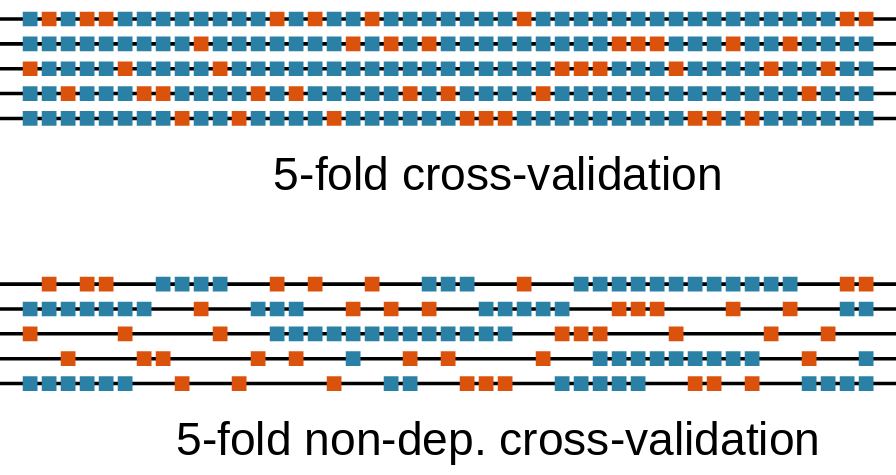
\includegraphics[width=0.7\linewidth]{Images/Cross-validation-scheme}
% 	\caption{$\mathcal{K}$-fold CV and $\mathcal{K}$-fold with non-dependent data. Observations in blue are used to estimation and in orange for evaluation. Note that non-dependent data does not use all dataset in each fold. Image from \cite{bergmeir_note_2017}.}
% 	\label{fig:cross-validation-scheme}
% \end{figure}
% In both settings, the training data is randomly split into a collection of sets $S_k$, forming a $\mathcal{K}$ size partition. Each of these $S_k$ is used as test set, while the rest is used to estimate coefficients which will be used to predict values of $S_k$. 
% As there are $\mathcal{K}$ folds, this procedure is done $\mathcal{K}$ times. 
% So, for a given vector of tuning parameter $\theta$, the CV score is given by the sum of the error function for each fold. 
% As the CV score is nonconvex, the optimization in (\ref{eq:cv-equation}) is done by iterating over a sequence of values in a thin grid and choosing the smallest one.




% Even though CV is very popular and produce great results, selecting model with Information Criteria involves less computational time. For the case where the selected model is very similar, it might be the case that the estimation methodology may change a little bit. It is definitely a topic that worths researching.


% \todoi{Ver se novas figuras (R/grafico-cv.r) e ver se incluir outras formas de CV} % escolhemos trabalhar apenas com este tipo de CV





\subsection{Monte Carlo scenario generation} \label{sec:scenario-generation}

This section presents how to generate future scenarios of time series $\{y_t\}$ from the estimated coefficients from a QR model using a Monte Carlo (MC) approach. 
%Let $|T|$ be the total length of $\{y_t\}$ and $S$ the number of scenarios of size $K$ we produce. 
%The variables chosen to compose $x_t$ can be either exogenous variables, autoregressive components of $y_t$ or both. We use a nonparametric approach which to estimate, at every $t$, the $k$-step ahead conditional density of $y_t$.
The MC procedure  we use to produce $S$ different future scenarios $\{ \hat{y}_{\tau,s} \}_{\tau=|T|+1}^{|T|+K}$ consists in first estimating the model for a given time $\tau$ and scenario $s$. Then, for each of these we take input vector $x_{\tau,s}$ and calculate the discrete quantile function $\tilde{Q}_{y_{\tau}|X}$, which is the intermediate step to estimate the continuous quantile function $\hat{Q}_{y_{\tau}|X}$. 
This same MC procedure is employed to produce scenario simulations for a variaty of QR based models, including the QRAL.

\noindent\rule{\columnwidth}{1pt}

MC procedure for simulating $S$ future scenarios of $\{y_{\tau,s}\}$

\noindent\rule{\columnwidth}{1pt}

\begin{enumerate}
	
	\item Estimate a QR model (for the QRAL solve the optimization problem defined in equation (\ref{eq:adaLASSO-1})-(\ref{eq:adaLASSO-ult})). 
	A set of coefficients $\{ \hat\beta_{0j} \}_{j \in J}$ and $\{ \hat\beta_{j} \}_{j \in J}$ is the output from this optimization, using time series $y_t$ and $x_{pt}$ from the period $t = 1, \dots, |T|$. 

	\item Initialize time index $\tau = |T| + 1$.
	
	\item For each scenario $s \in S$, do:
		\begin{enumerate}

		\item Let $x_{\tau,s} = [y_{\tau-1,s}, \dots, y_{\tau-24,s}]$ be the vector of explanatory variables used as input to predict the conditional distribution function in time $\tau$ and scenario $s$.

		\item Let $\tilde{Q}_{y_{\tau}|X}:A \times \mathbb{R}^d \rightarrow \mathbb{R}$ be the discrete quantile function. Its values are mapped according to the estimated quantile $\tilde Q_{y_{\tau}|X}(\alpha_j, x_{\tau,s}) \leftarrow \hat\beta_{0j} + \hat\beta_j^T x_{\tau,s}$, for all $j \in J$.
		
		\item In order to define the continuous function $\hat{Q}_{y_{\tau}|X}:[0,1] \times \mathbb{R}^d \rightarrow \mathbb{R}$ from $\tilde Q_{y_{\tau}|X}$, use linear interpolation connecting the points. As $0 < \alpha_1 < \cdots < \alpha_{|J|} < 1$, there are no quantile estimates for the intervals $[0,\alpha_1]$ and $[\alpha_{|J|},1]$. These gaps are filled by linearly extending the line that connects $\alpha_1$ to $\alpha_2$ on the left hand side and extending the line that connects $\alpha_{|J|-1}$ to $\alpha_{|J|}$ on the right hand side until the support $[0,1]$ is fully mapped.  

		% \item In any given period $\tau$, for every $\alpha \in A$, we estimate $q_{\alpha_{j}}$, for every $j \in J$.
		% Note that $x_{\tau}$ is supposed to be known at time $\tau$\footnote{In the presence of exogenous variables that are unknown, it is advisable to incorporate its uncertainty by considering different scenarios. In each scenario, though, $x_{\tau}$ must be considered fully known.}.
		
		% \item Let $\hat{Q}_{y_{\tau,s}|X}(\alpha,x_\tau)$ be the estimated quantile function of ${y}_{\tau,s}$. 
		% At first, we define a discrete quantile function $\tilde{Q}_{y_{\tau,s}}$. By mapping every $\alpha \in A$ with its estimated quantile $\hat{q}_{\alpha_j}(x_t)$, we define function $\tilde{Q}_{y_{\tau,s}}$. In order to produce a continuous function from a set of ordered points, we use linear interpolation and we arrive on the Quantile function $\hat{Q}_{y_{\tau}}$.
		
		%This process is described in more details on section \ref{sec:estimating-distribution}. 
		\item Let $U$ be a random variable with uniform distribution over the interval $[0,1]$. As $Q_{y_\tau}(U)$ has the same distribution as $y_\tau$, by taking
		$$y_{\tau,s} \leftarrow \hat Q_{y_\tau | X}(u), \quad u \sim U[0,1],$$
		we simulate scenarios next values.



		 \end{enumerate}
	% let $x_{\tau,s} = [y_{\tau-1,s}, \dots, y_{\tau-12,s}]$ be the vector of explanatory variables, used as input to predict the conditional distribution function in time $\tau$ and scenario $s$.
	
	
	\item Let $\tau = \tau + 1$. If $\tau > K$, then stop. Else, go back to step 3) . 


\end{enumerate}

\noindent\rule{\columnwidth}{1pt}


\subsection{Schwarz Information Criteria for Quantile Regression (SIC)} \label{sec:SIC}

Information criteria (IC) is the state of the art in time series model selection. It is also employed in other multiple quantile model studies \cite{zou_regularized_2008, jiang_interquantile_2014} to tune parameters.
An IC summarizes two desirable characteristics in model selection: in-sample goodness of fit and penalization of complexity as given by the model size. Hence, in order for a covariate to be included in the model, it must supply enough goodness of fit. The expression for SIC appropriate for quantile autoregression is presented below:
% {\small
% \begin{align} 
% \begin{split}
% SIC_m = \sum_{j \in J} \left( \log \left(\sum_{t \in T}\rho_{\alpha_j}(y_t - \beta_{0j} - \beta_j^T x_t) \right) +  \frac{\log(|T|)|\epsilon_j|}{2|T|}  \right),\label{eq:SIC}
% \end{split}					
% \end{align}} 
 \begin{equation} 
\small
SIC_\theta = \sum_{j \in J} \left( \log \left(\sum_{t \in T}\rho_{\alpha_j}(y_t - \beta_{0j}^\theta - \beta_j^{T\theta} x_t) \right) +  \frac{\log(|T|)|\epsilon_\theta|}{2|T|}  \right),\label{eq:SIC}
\end{equation}
where $\theta = [\gamma \quad \lambda]^T$ and $\epsilon_\theta$ is the elbow set, defined as $\epsilon_\theta = \{(t,j): y_t - q_{\alpha_j}(x_t) = 0 \}$. The authors in \cite{li_l1-norm_2008} show that the quantity $|\epsilon_\theta|$ is the effective degrees of freedom in the quantile regression.


\subsection{Model selection based on goodness of fit for scenarios (GFS)} \label{sec:GFS}

Most statistical models are designed to provide a good fit on point forecasts, but under the stationarity assumption produces scenarios which quickly converge to the unconditional mean.
The applications that use future scenarios, discussed in Section \ref{sec:introduction}, demands that these scenarios resemble the time series past behavior.
In order to produce scenarios that fit our goals, we must select the best statistical model according to this objective. 
% The usage of a measure of fitness that is popular to other applications, such as the $k$-step ahead forecasting error,  

We propose a novel metric, where we simulate future scenarios and take the mean absolute error (MAE) of the unconditional forecasted scenarios to select the model that produces scenarios most similar to those obtained from the observed data.
The appropriate version of MAE for quantile regression is defined by
\begin{equation}
MAE_{\theta}= \frac{1}{|J|} \frac{1}{12} \sum_{j \in J} \sum_{i = 1}^{12}  \left| q_i^{\alpha_{j}}- \hat q_i^{\alpha_{j}}  \right|,
\label{eq:MAE}
\end{equation}
where $q_t^{\alpha_{j}}$ is the unconditional $\alpha_j$-quantile  and $\hat q_t^{\alpha_j}$ the predicted $\alpha_j$-quantile. We obtain $q_t^{\alpha_j}$ by taking the $\alpha_j$-quantile of the historic values of a given month. The predicted $\hat q_t^{\alpha_j}$ is obtained by taking the $\alpha_j$-quantile 
The MAE error function emphasizes the accuracy across quantiles. Depending on the application, it might be interesting to put different weights on different quantiles. In this work, however, we will treat every quantile as equals concerning the error measure.

We consider the third year ahead as the time series unconditional state. Given that the observed values lies on $t \in \{1,\dots,|T| \}$, the subset of future scenarios $\{y_{|T|+25,s}, y_{|T|+26,s}, \dots, y_{|T|+36,s} \}$ is compared with the observed past values of each month. 
For each month $i = 1,\dots, 12$, take the $\alpha_j$-quantile $\hat q_t^{\alpha_j}$ from the set of $S$ scenarios $y_{|T|+24+i}$. The estimated quantile is compared with the historic quantile from this period. For example, we evaluate how close the 25\%-quantile
of all simulated scenarios in the month of March (from the third year) is against the 25\%-quantile
of all observed months of March. We take the MAE of the absolute difference $\left| q_i^{\alpha_{j}}- \hat q_i^{\alpha_{j}}  \right|$ for every month $i$ and quantile $j$ as the error measure, as shown on equation (\ref{eq:MAE}).

The output of problem (\ref{eq:adaLASSO-1})-(\ref{eq:adaLASSO-ult}) is the best 1-step ahead model, giving the tuning parameter $\lambda$ and $\gamma$. 
So, selecting tuning parameters according to realistic scenario generation puts together a goodness of fit for both the conditional $k$-step ahead, which produces reliable scenario on the short term, but also for scenario generated for the long term.  

% where $q_t^{\alpha_{j}}$ is the true $\alpha$-quantile from the data (in the case study, we use the monthly distribution as a good enough approximation of the true quantile, as RG time series such as wind power are stationary) and $\hat q_t^{\alpha_j}$ is the $\alpha$-quantile from these scenarios, when estimating the model with parameters $\lambda$ and $\gamma$.
% This function has the advantage of penalizing error proportionally to the quantile value it is estimating. 


% In order to evaluate the model performance, we need to define an error metric. The minimization of this error metric is the objective in estimating the statistical model. 
% As conditional distribution is the focus in this paper, 

% \todo{Voltar para essa seção}





%


%% ===== Sec. IV - Simulation ===== %

%\input{ieee-simulation.tex}

%% ===== Sec. V - Estimation ===== %
%
%\input{ieee-estimation.tex}


%% ===== Sec. VI - Case studies ===== %
%
\section{Case Studies}


\subsection{Controlled Studies I - Autoregressive Process} \label{sec:ar-study}


Firstly, the performance of QRAL methodology is evaluated by simulating the widely used autoregressive process and in the sequel estimating the QRAL framework to evaluate if it is capable to recover the parameters fixed at the beginning. 
The aforementioned autoregressive process is set as
\begin{equation}
y_t = \beta_1 y_{t-1} + \varepsilon_t, \quad \varepsilon_t \sim N(0, 1), \quad t=1,\dots,400 \label{eq:ar1}
\end{equation}
with length 400 and $\beta_1 = 0.3$. This value was chosen due to the fact that the sample size of RG time series have such length in general.

Three different methods were employed to estimate the process given by (\ref{eq:ar1}):
\begin{enumerate}
\item \textbf{Quantile Regularized Adaptive LASSO (QRAL)}, which estimates a different model for each quantile $Q_{y_t|X}(\alpha,\cdot)$, for all ${j \in J}$. In practice, it means that each coefficient $\beta_{1j}$ is estimated with regularization on each quantile. %As the QRAL estimates a different solution for all every $\alpha$-quantile of $y_t$, the model $$y_t^{\alpha_j} = \beta_{0\alpha_j} + \beta_{\alpha_j} y_{t-1}, \quad \text{for all } j \in J$$ will produce as output a different model for each probability quantile $y_t^{\alpha_j}$.
\item \textbf{Quantile Regression as Koenker (QRK)} as originally proposed by \cite{koenker1978regression}, where each coefficient $\beta_{1j}$ is estimated using QR. 
\item A simple \textbf{Autoregressive (AR)} process.%, the estimated model is $$y_t = \beta_0 + \beta_1 y_{t-1}, j \in J$$. As AR process is not a quantile  One coefficient for  the coefficients $\beta_p(\alpha)$ are all the same, for every quantile (AR(1) estimation).


\end{enumerate}

After simulate 1000 different time series given by Equation (\ref{eq:ar1}), $\beta_{1j}$ was estimated for each of the aforementioned models. Regarding parameter $\gamma$ (see Eq. (\ref{eq:adalasso-1})-(\ref{eq:adalasso-ult})) it was estimated using CV, as described in section \ref{sec:cv}. Since in this experiment the model has only one lag, model selection will not be evaluated, hence $\lambda=0$.

The main objective of this simulation experiment was to evaluate how our nonparametric methodology can correctly recover the true AR(1) process. The model performance was evaluated by examining how closely the estimated quantiles are from the populational ones. The results for each method are depicted in Figure \ref{fig:boxplot-ar1}, where a boxplot containing the results for the 1000 simulations is shown. %a single boxplot for AR(1) and one for each probability $\alpha$ for QRAL and QRK.
\begin{figure*}[h]
	\centering
	\centerline{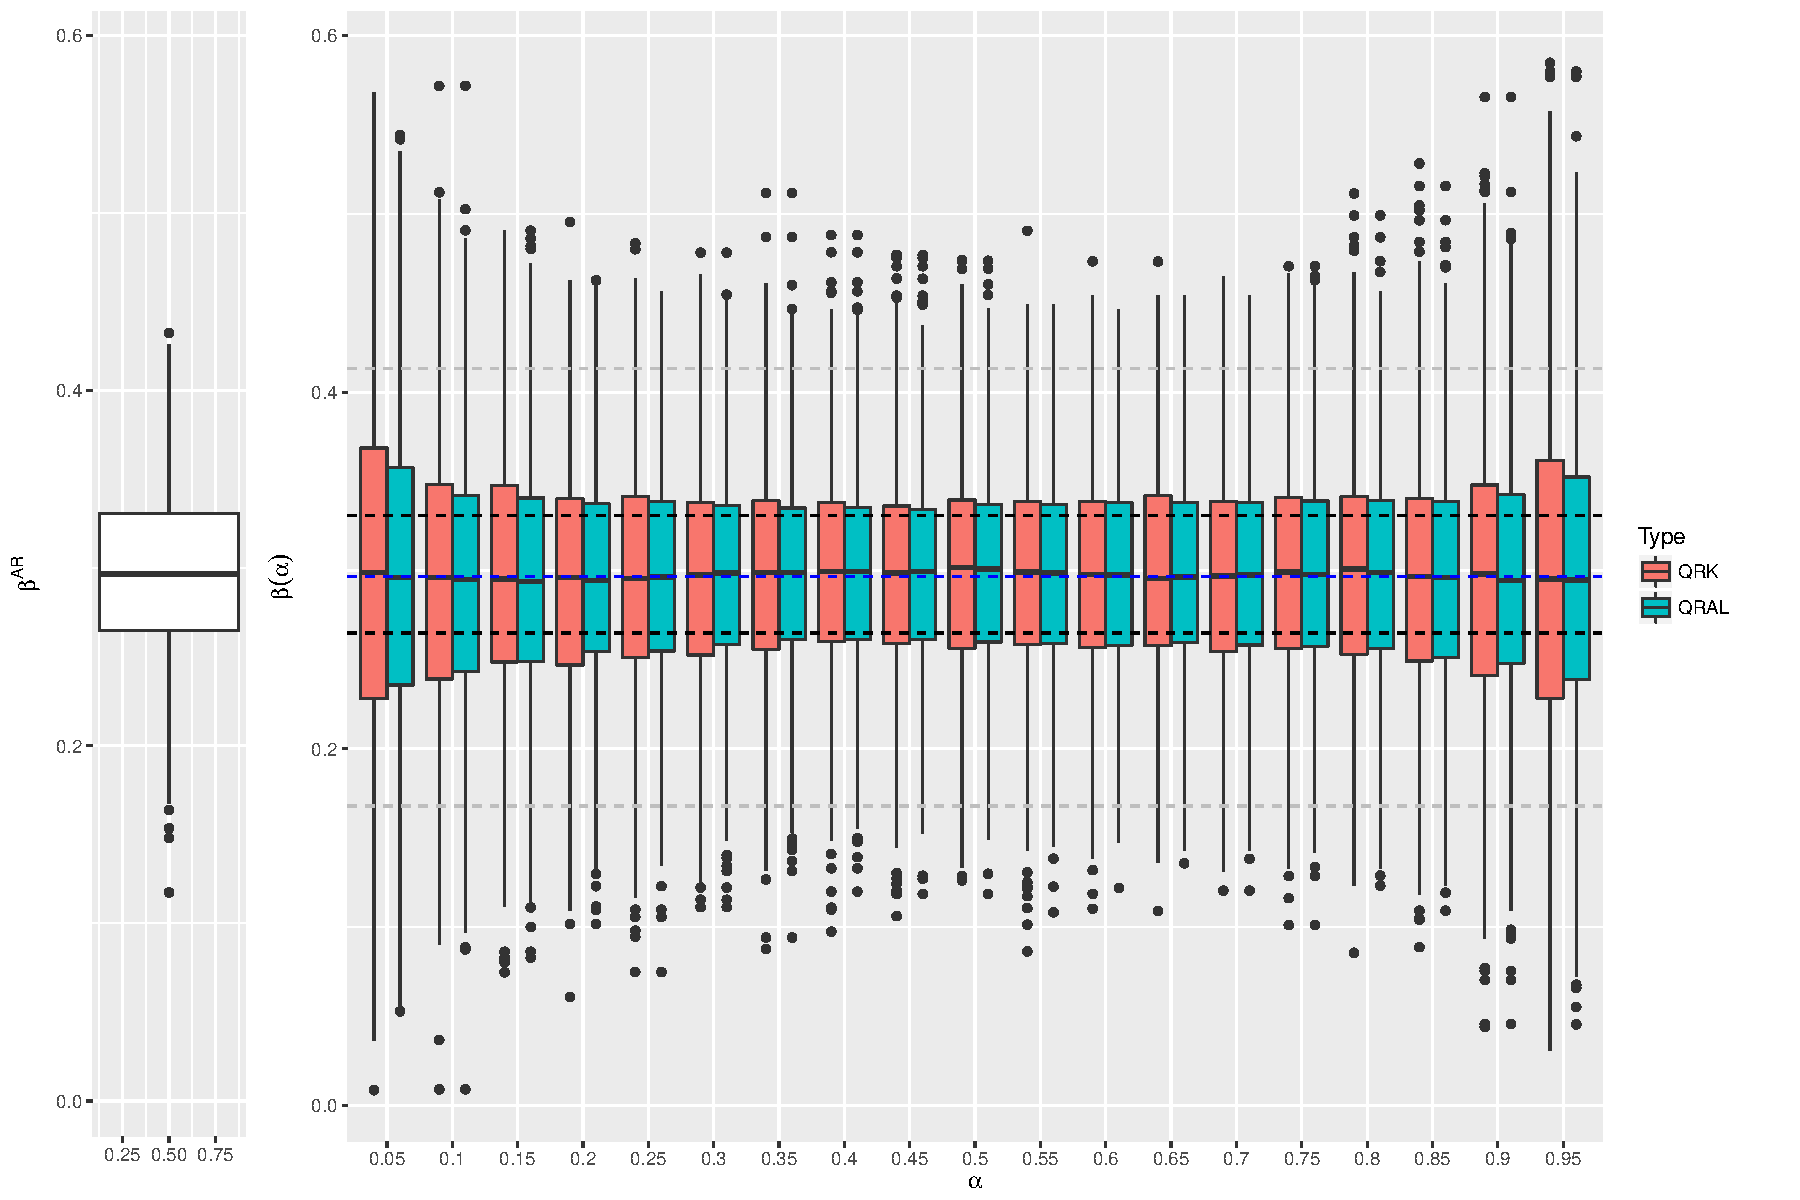
\includegraphics[width=7in]{Images/boxplot-ar1.pdf}}
	\caption{Boxplot showing estimated coefficient after 1000 iterations. On the left hand side, the boxplot of the AR(1) coefficient estimation. Note that for the AR(1) the coefficient is equal for all probabilities $\alpha$. On the right hand side, the boxplot of the regular QR (where $\gamma = 0$) and the QRAL where $\gamma$ is selected using cross-validation. }
	\label{fig:boxplot-ar1}
\end{figure*}
The conclusions from this experiment are: (i) Coefficient estimation errors for the central quantiles are not far from those estimated by the AR; (ii) extreme quantiles are usually harder to estimate, due to having fewer observations; as a consequence, the estimation error increases on the extremes (iii) QRAL has an advantage over QRK in terms of spread of estimators.


\section{Controlled Studies II - Quantile Autoregressive Process} \label{sec:qar-study}

In the second controlled study, the performance of QRAL is evaluated in a Quantile Autoregressive Process. While in the first study the time series $y_t$ is generated by a process with a coefficient $\beta_1$ constant across quantiles, in this experiment $\beta_1$ is a piecewise linear function of $\alpha$, described graphically on Figure \ref{fig:betas-qar}. 
\begin{figure}[h]
	\centering
	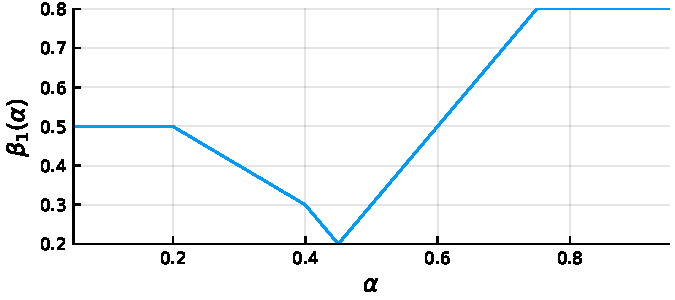
\includegraphics[width=0.6\linewidth]{Images/Betas-Qar.pdf}
	\caption{Coefficient $\beta_1(\alpha)$ of the Autoregressive term $y_{t-1}$ for generating the QAR process.}
	\label{fig:betas-qar}
\end{figure}

The simulation of a QAR process involves two steps. The first is to determine the values of $\beta_0$ from a set of values of $\beta_1(\alpha)$; the latter given as input. These values of $\beta_{0j}$ are the output of the following optimization problem:
\begin{IEEEeqnarray}{lr}
	\underset{\beta_{0}}{\text{min }} \beta_{0,|J|} - \beta_{0,1} \span \\
	\text{subject to} \span \\
	\beta_{0j} + \beta_{j}^T x_{t}  + h \leq \beta_{0,j+1} + \beta_{j+1}^T x_{t}, \span \nonumber  \\
	&\forall t \in T, \forall j \in J_{(-1)},
\end{IEEEeqnarray}
where $h$ is the minimum distance allowed between two neighbour quantiles. If $\beta(\alpha)$ is constant for an interval and $h$ is set to zero, this group of quantiles would superimpose one another. 
Once both vectors $\beta_0$ and $\beta_1$ are defined, the 1-step temporal dynamic of the process can be summarized by Figure \ref{fig:qar}. 

\begin{figure}[h]
	\centering
	\centerline{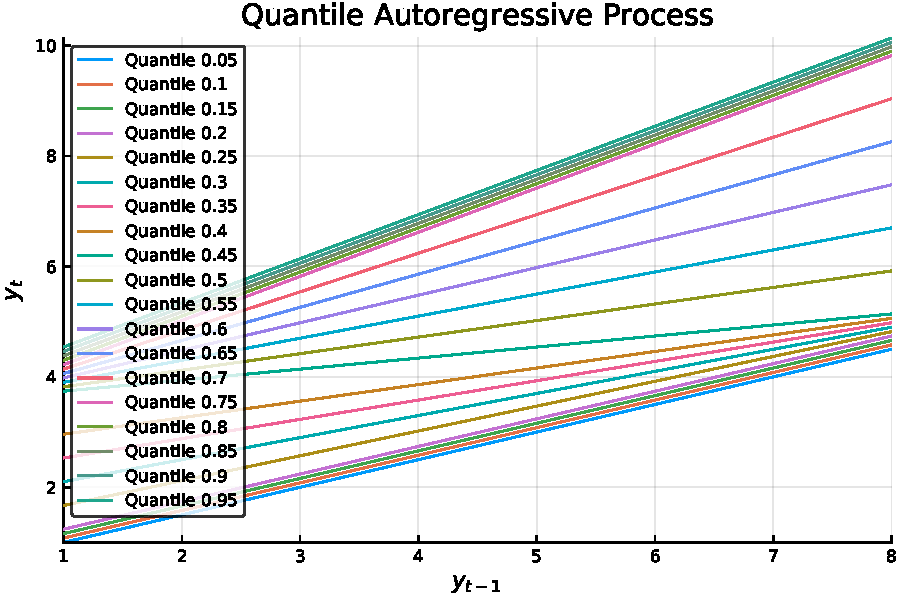
\includegraphics[width=0.8\linewidth]{Images/Qar.pdf}}
	\caption{Quantiles of $y_t$ vs $y_{t-1}$. For each given value of $y_{t-1}$ on the $x$-axis, the curves indicate different levels of quantiles for the values of $y_t$.}
	\label{fig:qar}
\end{figure}

The second step consists in simulate values of $y_t$. For a given value of $y_{t-1}$, the next term $y_t$ in the time series follows a distribution that can be constructed by the quantiles shown on Figure \ref{fig:qar}. 

This controlled study has the same sample setup as the one in the previous section: 1000 random samples of length 400 and the same three methods tested (QRAL, QRK and AR). The objective of this experiment is to test their performance with respect to their error on the estimation of each coefficient. The summary of results is given by Table \ref{tab:qar-results}, which shows the aggregated value of quadratic error across all $j \in J$.
The conclusion from this experiment is that both QR methods are much superior than an Autoregressive process such as a AR(1) when the coefficient $\beta$ is allowed to change with probability $\alpha$. 


\begin{table}[h]
\centering
\caption{Cumulated quadratic error of coefficient estimation for each method after 1000 random samples}
\label{tab:qar-results}
\begin{tabular}{lll}
\hline
AR(1) & QRAL & QRK   \\ \hline
38.75 & 5.039       & 5.314
\end{tabular}
\end{table}

\section{Case Study with realistic data}

In this section, the QRAL methodology is tested in generating future scenarios of RG. A real time series of Wind Power is the input for estimating coefficients that are employed to generate scenarios by using the procedure described on section \ref{sec:scenario-generation}.
The time series is composed of 31 years (from 1981 to 2011) of monthly observations  of a wind farm located in the Brazilian northeast, measured in megawatts. The yearly series is shown on Figure \ref{fig:icaraizinho-mensal}.
\begin{figure}[h]
\centering
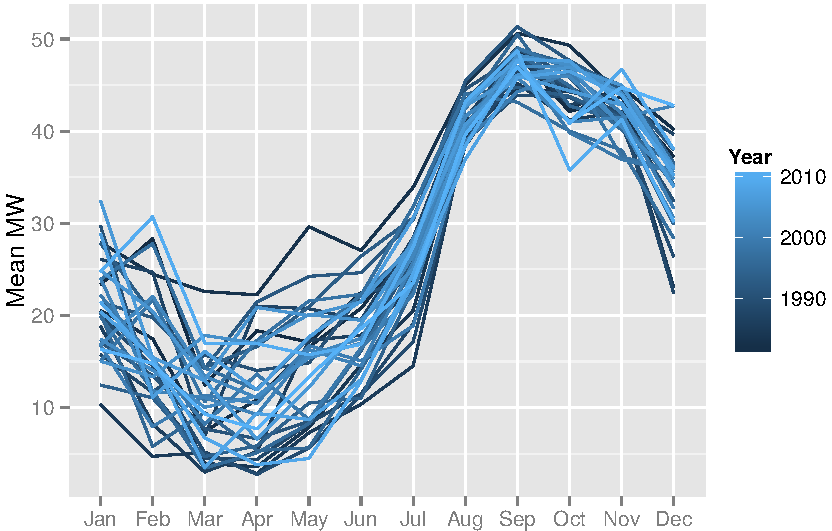
\includegraphics[width=0.8\linewidth]{Images/icaraizinho-mensal2}
\caption{Icaraizinho yearly data. Each serie consists of monthly observations for each year.}
\label{fig:icaraizinho-mensal}
\end{figure}

The last 4 years of this period are left as out-of-sample test data. Six different methods are used to generate scenarios: QRL (Quantile Regularized LASSO), QRAL, QRK, LASSO (original LASSO for QR), AdaLASSO (original AdaLASSO for QR) and SARIMA. The estimated coefficients for the QR based methods are presented on Figure \ref{fig:betas-icaraizinho}. 
\begin{figure*}[h]
	\centering
	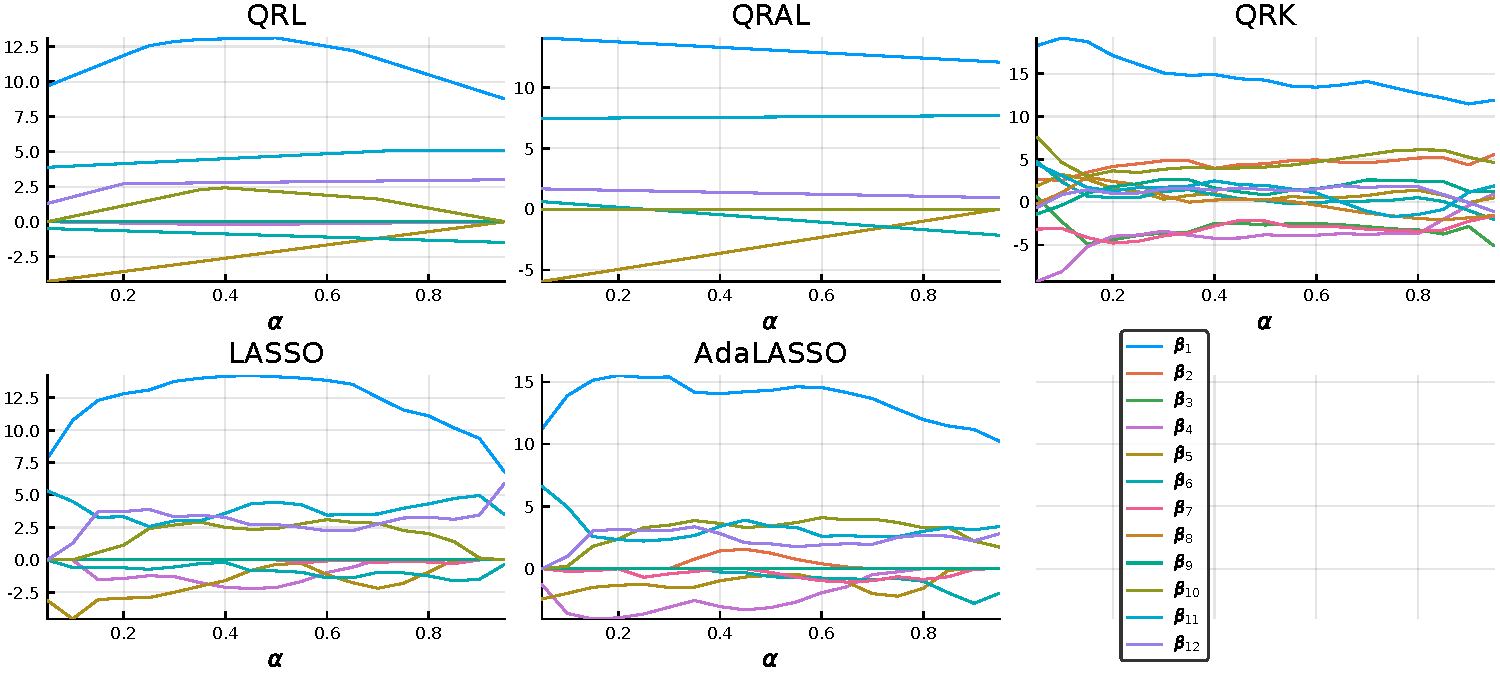
\includegraphics[width=1.0\linewidth]{Images/betas-icaraizinho}
	\caption{Estimated coefficients for each QR based methods. Each line represents the coefficient function $\beta_{p}$ for a given covariate $y_{t-p}$.}
	\label{fig:betas-icaraizinho}
\end{figure*}
The second derivative filter acts reducing the noise, and its effect can be seen clearly when comparing the estimated coefficients of QR-LASSO with the LASSO and the QRAL with the AdaLASSO. 

The accuracy of the generated scenarios - considering the MAPE metric - in recovering the historic quantiles for each month is the metric used for evaluation. These results are shown on Table \ref{tab:results-icaraizinho}. The QRAL is the method that produced the scenarios with the smaller errors.

\begin{table}[h]
\centering
\caption{Cumulated MAPE across all $\alpha_j$ quantiles}
\label{tab:results-icaraizinho}
\begin{tabular}{@{}llllll@{}}
\toprule
QRL & QRAL & QRK   & LASSO & AdaLASSO & SARIMA \\ \midrule
6.809    & 3.653       & 3.940 & 6.282 & 4.653    & 5.834 
\end{tabular}
\end{table}



%% ===== Sec. VI - Further Studies ===== %

%  \section{Further Studies}

The obtained results using the QR methodology give incentives to keep doing experiments and finding new aspects which could help improve the process of generating scenarios. Of the many possible paths, the following are the next steps to be investigated by the researchers. 

\subsection{Information Criteria for Quantile Regression}
Using CV can be computationally expensive, as the full estimation is done several times for each tuning parameter - in this case, $\gamma$ and $\lambda$. Other form of deciding the quantity of variables that provides a good equilibrium between in-sample prediction and parsimony is the Information Criteria.

Information criteria summarizes two aspects. One of them refers to how well the model fits the in-sample observations and the other part penalizes the quantity of covariates used in the model. By penalizing how big our model is, we prevent overfitting from happening. So, in order for a covariate to be included in the model, it must supply enough goodness of fit.
In \cite{machado1993robust}, it is presented a variation of the Schwarz criteria for M-estimators that includes quantile regression. The Schwarz Information Criteria (SIC), adapted to the quantile autoregression case, is presented below:
\begin{align} 
\begin{split}
SIC(m) = \sum_{j \in J} \log \left(\sum_{t \in T}\rho_{\alpha_j}(y_t - \beta_0 - \beta^T x_t) \right) +  \frac{\log|T|}{2|T||P|} K(m),\label{eq:SIC}
\end{split}					
\end{align}
where $K(m)$ is the quantity of coefficients $\beta_{pj}$ greater than zero in the model $m$.
By minimizing the $SIC$ function, the chosen model is the one with the best combination, according to this metric, of fit and parsimony among all models. 

Even though CV is very popular and produce great results, selecting model with Information Criteria is much quicker. For the case where the selected model is very similar, it might be the case that the estimation methodology may change a little bit. It is definitely a topic that worths researching.

\subsection{Quantile Autoregression with a nonparametric approach}
\label{sec:npqar}

Fitting a linear estimator for the Quantile Auto Regression is less efficient if nonlinearity is present in the quantile functions. This nonlinearity may produce a linear estimator that underestimates the quantile for a chunk of data while overestimating for the other chunk. To prevent this issue from occurring we propose to use a nonparametric quantile regression model. 
% To sprevent overfitting and smoothen our predictor, we include a penalty on its roughness by including the $\ell_1$ norm of its second derivative. For more information on the $\ell_1$ norm acting as a filter, one can refer to \cite{kim2009ell_1}.

% This time, as opposed to when employing linear models, we don't suppose any functional form for $q_\alpha(x_t)$. This forces us to build each $q_\alpha$ differently: instead of finding a set of parameters that fully defines the function, we find a value for $q_\alpha(x_t)$ at each instant $t$. On the optimization problem, we will find optimal values for a variable $q_{tj} \in \mathbb{R}$, each consisting of a single point. The sequence  $\{ q^*_{\alpha t} \}_{\alpha \in A} $ will provide a discretization for the quantile function $\hat{q}_\alpha(x_t)$, which can be found by interpolating these points.

% notação estatística de ordem. com x^(0)

Let $\{\tilde{y}_t \}_{t=1}^n$ be the sequence of observations in time $t$ and let $\tilde{x}_t$ be the $p-$lagged time series of $\tilde{y}_t$, such that $\tilde{x}_t = L^p(\tilde{y}_t)$, where $L$ is the lag operator. Matching each observation $\tilde{y}_t$ with its $p-$lagged correspondent $\tilde{x}_t$ produces $n-p$ pairs $\{(\tilde{y}_t,\tilde{x}_t)\}_{t=p+1}^n$ (note that the first $p$ observations of $y_t$ must be discarded). When the sequence of observations of $x$ are reorder in such a way that they are in growing order
$$\tilde{x}^{(p+1)} \leq \tilde{x}^{(p+2)} \leq \dots \leq \tilde{x}^{(n)},$$ 
the new sequences can be defined $\{x_i\}_{i=1}^{n-p} = \{\tilde{x}^{(t)} \}_{t=p+1}^{n}$ and $\{y_i\}_{i=1}^{n-p} = \{\tilde{y}^{(t)} \}_{t=p+1}^{n}$, where $T' = \{2,\dots, n-p-1\}$. 

The optimization model to estimate the nonparametric quantile is as follows:
\begin{equation}
\begin{split}
\hat{q}_{\alpha_j}(x_t) =\underset{q_{tj}}{\arg\min}\sum_{t\in T'} \rho_{\alpha_j} \left( y - q_{tj} \right) \\ +\lambda_1  \sum_{t\in T'}|D_{x_t}^{1}q_{tj}| +\lambda_2  \sum_{t\in T'}|D_{x_t}^{2}q_{tj}|,
\end{split}
\end{equation}
where $D^1 q_t$ and $D^2 q_t$ are the first and second derivatives of the $q_\alpha(x_t)$ function, calculated as follows:
\begin{equation*}
D_{x_{t}}^{2}q_{tj}=\frac{\left(\frac{q_{\alpha t+1}-q_{tj}}{x_{t+1}-x_{t}}\right)-\left(\frac{q_{tj}-q_{\alpha t-1}}{x_{t}-x_{t-1}}\right)}{x_{t+1}- x_{t-1}},
\end{equation*}

\begin{equation*}
D^{1}_{tj}=\frac{q_{\alpha t+1}-q_{tj}}{x_{t+1}-x_{t}}.
\end{equation*}
%The first part on the objective function is the usual quantile regression condition for $\{q_{t\alpha}\}_{\alpha \in A}$. The second part is the $\ell_1$-filter. The purpose of a filter is to control the amount of variation for our estimator $q_\alpha(x_t)$. When no penalty is employed we would always get $q_{tj} = y_t$, for any given $\alpha$. On the other hand, when $\lambda_2 \rightarrow \infty$, our estimator approaches the linear quantile regression. 

The full model can be rewritten as a LP problem as bellow:
\begin{IEEEeqnarray}{lcr}
\min_{q_{tj},\varepsilon^+_{tj}, \varepsilon_{tj}^-, \xi_t} & \sum_{j \in J} \sum_{t \in T'}\left({\alpha_j}\varepsilon_{tj}^{+}+(1-{\alpha_j})\varepsilon_{tj}^{-}\right) & \\
& \qquad \qquad \qquad \qquad \qquad + \lambda_1\sum_{t \in T'}\gamma_{tj} + \lambda_2\sum_{t \in T'}\xi_{tj} & \nonumber \\
s.t. & \varepsilon_{t}^{+}-\varepsilon_{tj}^{-}=y_{t}-q_{tj}, & \qquad\forall t \in T',\forall j \in J,\\
   & D^{1}_{tj}=\frac{q_{\alpha t+1}-q_{tj}}{x_{t+1}-x_{t}},
    & \qquad\forall t \in T',\forall j \in J,\\   
 & D^{2}_{tj}=\frac{\left(\frac{q_{\alpha t+1}-q_{tj}}{x_{t+1}-x_{t}}\right)-\left(\frac{q_{tj}-q_{\alpha t-1}}{x_{t}-x_{t-1}}\right)}{x_{t+1}- x_{t-1}}.
  & \qquad\forall t \in T',\forall j \in J,\\
 & \gamma_{t \alpha}\geq D^1_{tj}, & \qquad\forall t \in T',\forall j \in J,\\
  & \gamma_{t \alpha}\geq-D^1_{t \alpha}, & \qquad\forall t \in T',\forall j \in J,\\
  & \xi_{t \alpha}\geq D^2_{tj}, & \qquad\forall t \in T',\forall j \in J,\\
 & \xi_{t \alpha}\geq-D^2_{t \alpha}, & \qquad\forall t \in T',\forall j \in J,\\
 & \varepsilon_{t \alpha}^{+},\varepsilon_{t \alpha}^{-},\gamma_{t \alpha}, \xi_{t \alpha}\geq0, & \qquad\forall t \in T',\forall j \in J,\\
  & q_{t j} \leq q_{t j+1}, & \qquad \forall t \in T', \forall j \in J_{(-1)}
  \end{IEEEeqnarray}


The output of this optimization problem is a sequence of ordered points $\{(x_t, q_{tj})\}_{t \in T}$, for all $j \in J$. The next step is to interpolate these points in order to provide an estimation for any other value of $x_t$. To address this issue, we propose using a linear interpolation. Note that $q_{tj}$ is a variable that represents only one point of the $\alpha_j$-quantile function $q_\alpha(x_t)$. 

The quantile estimation is done for different values of $\lambda_2$. By using different levels of penalization on the second difference, the estimation can be more or less adaptive to the fluctuation. It is important to notice that the usage of the $\ell_1$-norm as penalty leads to a piecewise linear solution $q_{tj}$. % Referenciar?
Figure \ref{fig:npqar-results} shows the quantile estimation for a few different values of $\lambda_2$. 

	
% Para os gráficos antigos, usar a pasta /npqar/
\begin{figure*}[htp]
  \centering
  \begin{minipage}[t]{0.4\linewidth}
    \centering
    \begin{minipage}[t]{\linewidth}
      \centering     \includegraphics[width=\textwidth]{Figuras-DocRQ/icaraizinho-crossing-01}
      \subcaption{$\lambda_1 = 0, \, \lambda_2 = 0.1$}
    \end{minipage}
    \begin{minipage}[b]{\linewidth}
      \centering     \includegraphics[width=\textwidth]{Figuras-DocRQ/icaraizinho-crossing-03}
      \subcaption{$\lambda_1 = 0, \, \lambda_2 = 0.3$}
    \end{minipage}
     \begin{minipage}[b]{\linewidth}
      \centering     \includegraphics[width=\textwidth]{Figuras-DocRQ/icaraizinho-crossing-1}
      \subcaption{$\lambda_1 = 0, \, \lambda_2 = 1$}
     \end{minipage}
  \end{minipage}
  \begin{minipage}[t]{0.4\linewidth}
    \centering
    \begin{minipage}[t]{\linewidth}
      \centering     \includegraphics[width=\textwidth]{Figuras-DocRQ/icaraizinho-crossing-3}
      \subcaption{$\lambda_1 = 0, \, \lambda_2 = 3$}
    \end{minipage}
    \begin{minipage}[b]{\linewidth}
      \centering     \includegraphics[width=\textwidth]{Figuras-DocRQ/icaraizinho-crossing-10}
      \subcaption{$\lambda_1 = 0, \, \lambda_2 = 10$}
    \end{minipage}
     \begin{minipage}[b]{\linewidth}
      \centering     \includegraphics[width=\textwidth]{Figuras-DocRQ/icaraizinho-crossing-200}
      \subcaption{$\lambda_1 = 0, \, \lambda_2 = 200$}
      \label{fig:npqar-cross}
     \end{minipage}
  \end{minipage}
  \caption{Quantile estimations for a few different values of $\lambda_2$. The quantiles represented here are $\alpha = (5\%, 10\%, 25\%, 50\%, 75\%, 90\%, 95\%)$. When $\lambda_2 = 0.1$, on the upper left, we see a overfitting on the estimations. The other extreme case is also shown, when $\lambda_2=200$ the nonparametric estimator converges to the linear model.}
  \label{fig:npqar-results}
\end{figure*}

%The first issue is how to select an appropriate value for $\lambda_2$. A simple way is to do it by inspection, which means to test many different values and pick the one that suits best our needs by looking at them. The other alternative is to use a metric to which we can select the best tune. We can achieve this by using a cross-validation method, for example.

%The other issue occurs when we try to add more than one lag to the analysis at the same time. This happens because the problem solution is a set of points that we need to interpolate. This multivariate interpolation, however, is not easily solved, in the sense that we can either choose using a very naive estimator such as the K-nearest neighbors or just find another method that is not yet adopted for a wide range of applications.





%% ===== Sec. - Conclusion ===== %
%
\section{Concluding Remarks}

In this work, we propose a nonparametric methodology based on QR to build the CDF of wind time series.  A linear model with regularization both on the quantile and on the covariates to produce future scenarios of RG, while the other is nonparametric on the quantiles and flexible enough to capture a nonlinear relation with the covariates. These scenarios are input for various applications in power systems and are essential in measuring risk in energy trading, planning the expansion of the energy systems and the dispatch problem. The nonparametric framework for estimating the CDF is specially useful when the data is not distributed according to a known distribution. 
Our methodology is capable of producing scenarios with distribution quality criteria on the estimation phase.  
These approach generated good quality scenarios that outperformed other known benchmarks, both in the QR literature (the Koenker model) as in the classic time series framework (SARIMA). 
The results obtained in this work brings incentives to continue researching methods for nongaussian time series, as they are present in many real world applications. 

%% ===== Sec. - Appendix ===== %
%
%\input{ieee-apendix.tex}

% % 

\bibliographystyle{IEEEtran}
\bibliography{Thesis,QR,Bibhenriquinho}



\end{document}
